%\documentclass[dvipdfmx]{beamer}      % platex の場合
\documentclass{beamer}                 % lualatex の場合
\usepackage{mySld}
\usepackage{multicol}

\begin{document}
\title{基礎コンピュータ工学\\第5章 機械語プログラミング\\(パート11)}
\date{}

\begin{frame}
  \titlepage
  \centerline{\url{https://github.com/tctsigemura/TecTextBook}}
  \vfill
  \centerline{本スライドの入手:
    \raisebox{-7mm}{
\includegraphics[scale=0.3]{../Img/QRs5_B.png}}}
\end{frame}

%==============================================================================
%\begin{frame}
%  \frametitle
%  \tableofcontents
%\end{frame}

\section{アドレッシングモード}
%==============================================================================
\begin{frame}
  \frametitle{アドレッシングモード}
  LD,ST,ADD,SUB,CMP,AND,OR,XOR,JMP,JZ,\\
  JC,JM,JNZ,JNC,JNMの命令フォーマットは同じだった.
  \twoByte{\OP}{\GR~\XR}{\A}

  これまで,\emph{XRフィールドは$00_2$}にしてきた.\\
  XRフィールドは,
  メモリデータのアドレス計算方法を決める\\
  \emph{アドレッシングモード}を指定する.\\

  {\small\begin{center}
    \begin{tabular}{c|l l}
      \hline
      \hline
      XR & \multicolumn{2}{|c}{意味} \\
      \hline
      $00_2$ & ダイレクトモード     & (直接モード)   \\
      $01_2$ & G1インデクスドモード & (G1指標モード) \\
      $10_2$ & G2インデクスドモード & (G2指標モード) \\
      $11_2$ & イミディエイトモード & (即値モード)   \\
    \end{tabular}
  \end{center}}
  \vfill
  \vfill
\end{frame}

%==============================================================================
\begin{frame}
  \frametitle{ダイレクト(直接)モード}
  これまで使用してきた\emph{アドレッシングモード}は\emph{ダイレクトモード}
  \vfill
  \begin{itemize}
  \item \emph{実効アドレス(EA : Effective Address)} \\
    実効アドレス = 第2バイトの内容 \\
    \vfill
  \item \emph{XRフィールド=$00_2$}
    \vfill
  \item \emph{ニーモニック例} \\
    {\ttfamily\vspace{-0.5cm}\begin{center}
      \begin{tabular}{l l}
        LD & G0,A \\
        ST & G0,B \\
      \end{tabular}
    \end{center}}
    \vfill
  \item \emph{フローチャート例} \\
    \vspace{-0.5cm}\centerline{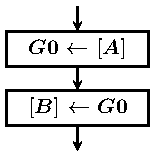
\includegraphics[scale=0.8]{../Tikz/flowE.pdf}}
  \end{itemize}
  \vfill
  \emph{実効アドレス} = 命令の操作対象となるメモリアドレスのこと.
  \vfill
\end{frame}

%==============================================================================
\begin{frame}
  \frametitle{インデクスド(指標)モード}
  G1,G2が配列データをアクセスするために使用できる.\\
  (\emph{G0,SPは使用できないので注意!!})
  \vfill
  \begin{itemize}
  \item \emph{実効アドレス(EA : Effective Address)} \\
    実効アドレス = 第2バイトの内容+G1の内容 \\
    実効アドレス = 第2バイトの内容+G2の内容 \\
    (この時,G1,G2は\emph{インデクスレジスタ}と呼ばれる.)
    \vfill
  \item \emph{XRフィールド(G1=$01_2$,G2=$10_2$)}
    \vfill
  \item \emph{ニーモニック例} \\
    {\ttfamily\vspace{-0.5cm}\begin{center}
      \begin{tabular}{l l}
        LD & G0,A,G1 \\
        ST & G0,B,G2 \\
      \end{tabular}
    \end{center}}
    \vfill
  \item \emph{フローチャート例} \\
    \vspace{-0.5cm}\centerline{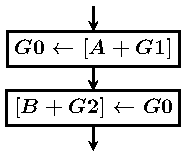
\includegraphics[scale=0.8]{../Tikz/flowF.pdf}}
  \end{itemize}
  \vfill
  \vfill
\end{frame}

%==============================================================================
\begin{frame}
  \begin{itemize}
  \item \emph{機械語の例(LD命令)} \\
    {\ttfamily\vspace{-0.7cm}\begin{center}
      \begin{tabular}{l l}
        LD & G0,A,G1 \\
      \end{tabular}
    \end{center}}
    \twoByte{0001}{00~01}{\A}
    \vfill
  \item \emph{機械語の例(ST命令)} \\
    {\ttfamily\vspace{-0.7cm}\begin{center}
      \begin{tabular}{l l}
        ST & G0,A,G2 \\
      \end{tabular}
    \end{center}}
    \twoByte{0010}{00~10}{\A}
    \vfill
  \item \emph{機械語の例(レジスタ)} \\
    {\ttfamily\vspace{-0.7cm}\begin{center}
      \begin{tabular}{l l}
        LD & G2,A,G1 \\
      \end{tabular}
    \end{center}}
    \twoByte{0001}{10~01}{\A}
  \vfill
  \end{itemize}
  \vfill
  \vfill
\end{frame}

%==============================================================================
\begin{frame}
  \frametitle{インデクスモードの使用例}
  配列AのI番目のデータ(\texttt{A[I]})をXにコピーする.
  \vfill
  \begin{minipage}[]{0.58\columnwidth}
  {\small\ttfamily\begin{center}
    \begin{tabular}{|l|l|l|l l|} \hline
      {\footnotesize 番地} & {\footnotesize 機械語} &
      {\footnotesize ラベル} & \multicolumn{2}{|c|}{ニーモニック} \\
      \hline
      00 & 14 07 &   & LD   & G1,I          \\
      02 & 11 08 &   & LD   & G0,A,G1       \\
      04 & 20 0B &   & ST   & G0,X          \\
      06 & FF    &   & HALT &               \\
      07 & 01    & I & DC   & 1             \\
      08 & 08    & A & DC   & 8             \\
      09 & 02    &   & DC   & 2             \\
      0A & 0A    &   & DC   & 10            \\
      0B & 00    & X & DS   & 1             \\
      \hline
    \end{tabular}
  \end{center}}
  \end{minipage}
  \begin{minipage}[b]{0.38\columnwidth}
    \twoByte{0001}{00~01}{0000~1000}
    \vspace{1.3cm}
  \end{minipage}
  \vfill
\end{frame}

%==============================================================================
\begin{frame}
  \frametitle{イミディエイト(即値)モード}
  命令の第2バイトがデータそのものになる.\\
  ZERO,ONE 等のデータを準備しなくても\emph{即値}を使用できる.\\
  (\emph{ST命令やジャンプ命令では使用できない.})\\
  \vfill
  \begin{itemize}
  \item \emph{実効アドレス(EA : Effective Address)} \\
    実効アドレス = 第2バイト \\
    \vfill
  \item \emph{XRフィールド = $11_2$}
    \vfill
  \item \emph{ニーモニック例} \\
    {\ttfamily\vspace{-0.5cm}\begin{center}
      \begin{tabular}{l l}
        LD & G0,\#1 \\
        LD & G0,\#A \\
      \end{tabular}
    \end{center}}
    \texttt{\#A}は,Aの内容ではなく,\emph{Aのアドレス}の意味!!
    \vfill
  \item \emph{フローチャート例} \\
    \vspace{-0.5cm}\centerline{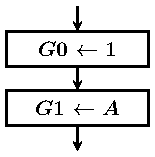
\includegraphics[scale=0.8]{../Tikz/flowG.pdf}}
  \end{itemize}
  \vfill
  \vfill
\end{frame}

%==============================================================================
\begin{frame}
  \begin{itemize}
  \item \emph{機械語の例(データの1)} \\
    {\ttfamily\vspace{-0.7cm}\begin{center}
      \begin{tabular}{l l}
        LD & G0,\#1 \\
      \end{tabular}
    \end{center}}
    \twoByte{0001}{00~11}{0000~0001}
    \vfill
  \item \emph{機械語の例(アドレスA)} \\
    {\ttfamily\vspace{-0.7cm}\begin{center}
      \begin{tabular}{l l}
        LD & G1,\#A \\
      \end{tabular}
    \end{center}}
    \twoByte{0010}{01~11}{\A}
  \item \emph{イミディエイトなし・ありの比較} \\
  \end{itemize}
  \begin{minipage}{0.48\columnwidth}
    \centerline{\ttfamily\begin{tabular}{|l l l|}\hline
           & ... &          \\
           & LD  & G0,ZERO  \\
           & ADD & G0,ONE   \\
           & ... &          \\
      ZERO & DC  & 0        \\
      ONE  & DC  & 1        \\\hline
    \end{tabular}}
  \end{minipage}
  \begin{minipage}{0.48\columnwidth}
    \centerline{\ttfamily\begin{tabular}{|l l l|}\hline
           & ... &          \\
           & LD  & G0,\#0  \\
           & ADD & G0,\#1   \\
           & ... &          \\
           &     &          \\
           &     &          \\\hline
    \end{tabular}}
  \end{minipage}
  \vfill
  \vfill
\end{frame}

%==============================================================================
\begin{frame}
  \frametitle{イミディエイトモードの使用例}
  A番地のデータに1を加えB番地に格納する.
  \vfill
  \begin{minipage}[]{0.58\columnwidth}
  {\small\ttfamily\begin{center}
    \begin{tabular}{|l|l|l|l l|} \hline
      {\footnotesize 番地} & {\footnotesize 機械語} &
      {\footnotesize ラベル} & \multicolumn{2}{|c|}{ニーモニック} \\
      \hline
      00 & 10 07 &   & LD   & G0,A      \\
      02 & 33 01 &   & ADD  & G0,\#1    \\
      04 & 20 08 &   & ST   & G0,B      \\
      06 & FF    &   & HALT &           \\
      07 & 05    & A & DC   & 5         \\
      08 & 00    & B & DS   & 1         \\
      \hline
    \end{tabular}
  \end{center}}
  \end{minipage}
  \begin{minipage}[b]{0.38\columnwidth}
    \twoByte{0011}{00~11}{0000~0001}
    \vspace{1.3cm}
  \end{minipage}
  \vfill
\end{frame}

%==============================================================================
\begin{frame}
  \frametitle{アドレッシングモードの使用例}
  A番地のデータでB番地からの\emph{10バイトの配列}を初期化する.
  \vfill
  \begin{minipage}{0.58\columnwidth}
    {\small\ttfamily\begin{center}
      \begin{tabular}{|l|l|l|l l|} \hline
        番地 & 機械語 & ラベル & \multicolumn{2}{|c|}{ニーモニック} \\
        \hline
        00 & 10 11 &      & LD   & G0,A          \\
        02 & 17 0A &      & LD   & G1,\#10       \\
        04 & 1B 00 &      & LD   & G2,\#0        \\
        06 & 22 12 & LOOP & ST   & G0,B,G2       \\
        08 & 3B 01 &      & ADD  & G2,\#1        \\
        0A & 47 01 &      & SUB  & G1,\#1        \\
        0C & A4 10 &      & JZ   & STOP          \\
        0E & A0 06 &      & JMP  & LOOP          \\
        10 & FF    & STOP & HALT &               \\
        11 & AA    & A    & DC   & 0AAH          \\
        12 & 00 00 & B    & DS   & 10            \\
        14 & 00 00 &      &      &               \\
        16 & 00 00 &      &      &               \\
        18 & 00 00 &      &      &               \\
        1A & 00 00 &      &      &               \\
        \hline
      \end{tabular}
    \end{center}}
  \end{minipage}
  \begin{minipage}{0.38\columnwidth}
    \centerline{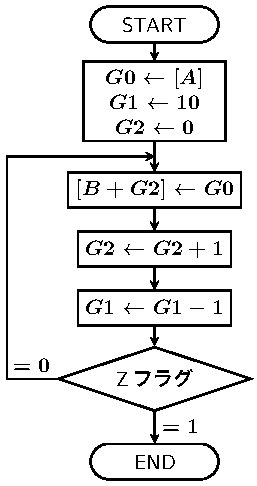
\includegraphics[scale=0.7]{../Tikz/flowD.pdf}}
  \end{minipage}
  \vfill
  \vfill
\end{frame}

%==============================================================================
\begin{frame}
  \frametitle{まとめ}
  \emph{学んだこと}
  \begin{itemize}
  \item 「\emph{実効アドレス(EA)}」 = 「データのメモリアドレス」
  \item 「アドレッシングモード」=「\emph{実効アドレス}の計算方法」
  \item TeCでは次のアドレッシングモードが使用できる.
    \begin{enumerate}
    \item[(1)] \emph{ダイレクト(直接)モード} \\
      「命令の第2バイトの内容」が実効アドレス
    \item[(2)] \emph{インデクスド(指標)モード} \\
      「命令の第2バイトの内容+レジスタの内容」が実効アドレス \\
      (アドレス計算には,G1,G2レジスタ\emph{だけ}が使用できる.)
    \item[(3)] \emph{イミディエイト(即値)モード} \\
      「命令の第2バイト」が実効アドレス
    \end{enumerate}
  \end{itemize}
  \vfill
  \emph{演習}
  \begin{itemize}
  \item イミディエイトモードのST命令をTeCで実行してみる.
  \item A番地からの5バイトのデータの和をB番地に求める.
  \item A番地からの5バイトのデータをB番地から5バイトにコピーする.
  \end{itemize}
  \vfill
\end{frame}

\end{document}
